\documentclass{article}
\usepackage[utf8]{inputenc}
\usepackage[russian]{babel}
\usepackage{amsmath}

\begin{document}

\subsubsection{Суть игрового процесса}
    Игровой процесс в данной игре представляет собой захватывающее сочетание платформера и стратегии, где игроку предстоит пройти через пять уникальных уровней, каждый из которых соответствует различным аспектам учебной программы «Компьютерные науки и технологии». Игрок берет на себя роль студента, который сталкивается с агрессивными врагами, представляющими собой дисциплины, предметы и приложения, стремящиеся помешать его успеваемости.\par
    Основные элементы игрового процесса:\par
    \begin{enumerate}
    \item \textbf{Платформенные элементы} \par
    Игроку предстоит прыгать, избегать препятствий и сражаться с врагами, используя свою ловкость и внимательность. Прыжки сверху на врагов — ключевой способ их уничтожения.
    \item\textbf{Стратегия и выбор пути} \par
    Игрок должен разрабатывать свою стратегию на каждом уровне, выбирая наиболее эффективный путь для достижения цели. Это включает в себя анализ препятствий и врагов, а также принятие решений о том, как лучше всего использовать свои навыки.
    \item \textbf{Система оценок} \par
    За успешное преодоление уровней и уничтожение врагов игрок получает «десятки», которые служат не только для прохождения на следующий уровень, но и как символ успеха и знаний игрока.
    \item \textbf{Разнообразие врагов и препятствий} \par
    Каждый уровень предлагает уникальных врагов и препятствий, что делает игровой процесс разнообразным и увлекательным. Игрок сталкивается с различными тактиками и подходами для победы над каждым видом противника.
    \end{enumerate}
    Игрок получает удовольствие от сочетания динамичного игрового процесса, стратегического мышления и возможности видеть свой прогресс, переходя с одного уровня на другой. Игра не только развлекает, но и позволяет глубже понять трудности и радости студенческой жизни.

\subsubsection{Ход игры и сюжет}
    \\Игровой сеанс начинается с того, что игрок погружается в мир Высшей Школы Экономики, где он играет за студента, который оказался в странной реальности, где учебные дисциплины и предметы стали врагами. Сюжет игры разворачивается через пять уровней, каждый из которых представляет собой отдельный курс обучения.\par
    В финале игрок сражается с дипломом, который использует все механики из предыдущих уровней. Эта битва требует от игрока максимальной концентрации, стратегического мышления и применения всех навыков, которые он приобрел на протяжении игры.\par
    После победы над дипломом игрок получает видит, как его знания и навыки применяются в реальной жизни на самом деле. Концовка игры заставляет задуматься о пройденном пути, подчеркивая важность образования и преодоления трудностей, с которыми сталкиваются студенты.
    Игрок выходит из игры с чувством удовлетворения и понимания, что обучение — это не только трудности, но и достижения.

\subsection{Физическая модель}
    \begin{itemize}
    \item \textbf{Физической модели игрового мира} \par
    Физическая модель игрового мира базируется на упрощенной физике, которая делает управление персонажем интуитивно понятным и отзывчивым для игрока. Основные законы физики такие, как гравитация и т.п., адаптированы для создания ощущения плавного и предсказуемого взаимодействия между персонажем, объектами и окружением.
    \item \textbf{Перемещение} \par
    Персонаж может перемещаться влево или вправо с постоянной максимальной скоростью, достигая её плавно (ускорение). Также, как и почти во всех играх такого типа, реализована механика прыжков, которые подчиняется параболической траектории и высотой которых можно управлять с помощью зажатия клавиши прыжка.
    \item \textbf{Боевые действия} \par
    Прыжок сверху на врага — это базовая атака, которая уничтожает или обезвреживает большинство врагов. Это ключевая механика, которая является простой для освоения, которая при этом может быть достаточно сложная в реализации для определенных противников.
    \end{itemize}

\subsection{Персонаж игрока}
    \begin{itemize}
    \item \textbf{Персонаж игрока - студент Высшей школы экономики} \\
    Данный персонаж - добрый, замотированный в учебе и преодолении различных сложностей во время учебного процесса студент. Он готов справляться с ними во что бы то ни стало и не опускать руки. На персонаже футболка из мерча Высшей школы эномики с надписью "HSE" для поддержания корпоративного стиля ВУЗа. В качестве цвета футболки выбран синий - самый узнаваемый цвет из брендбука ВШЭ, с которым знаком каждый студент Вышки. 
    \end{itemize}
\subsection{Элементы игры}
    Игра представляет из себя платформер с элементами roguelike — это жанр компьютерных игр, который сочетает в себе элементы двух  жанров: платформера и roguelike.  

    \begin{enumerate}
	\item \textbf{Противники} \par
	На каждом уровне игрок сталкивается с уникальными врагами, которые требуют разных подходов для победы над ними.
	Противники подразделяются на классы:
	\begin{itemize}
		\item \textbf{Противники ближнего боя:} \par
			Итеграл, философия
		\item \textbf{Противники дальнего боя:} \par
			SmartLMS, python, ворона, Яндекс.Почта
        \item \textbf{Боссы:} \par
            Диплом
	\end{itemize}
   Каждый из этих противников олицетворяет собой одну из трудностей, с которыми сталкиваются студенты Высшей школы экономики на пути к выпуску.
    \item \textbf{Уровни} \par
 Каждый уровень представляет собой отдельный курс обучения. Игра состоит из пяти уровней, и на каждом из них игрока ждут разнообразные противники и уникальное расположение игровых элементов.
    \item \textbf{Игровые элементы} \par
    \begin{itemize}
		\item Препятствия, ловушки
		\item Платформы, являющиеся основной составляющей уровней.
	\end{itemize}
    \item \textbf{Сложность} \par
    С каждым уровнем сложность игры повышается, а поведение врагов становится более непредсказуемым. Это заставляет игрока постоянно осваивать новые игровые механики, что поддерживает интерес к игре. 
    \item \textbf{Награды и достижения} \par
   За каждый пройденный уровень игрок получает достижение, которое можно сравнить с высшей оценкой в университетской шкале — «10».
   \end{enumerate}
\subsection{«Искусственный интеллект»}
    Искусственный интеллект (AI) в игре разработан так, чтобы создавать атмосферу, отражающую реальные студенческие трудности, при этом оставаясь простым и понятным для игрока.

\textbf{Общие принципы поведения AI:}

\begin{enumerate}
    \item \textbf{Противники ближнего боя:}  
    Эти враги, такие как интеграл или значок Яндекс.Почты, патрулируют ограниченные территории. Если игрок попадает в зону их действия, они начинают преследование. При уходе игрока за пределы зоны враги возвращаются к своему маршруту.  

    \item \textbf{Противники дальнего боя:}  
    Например, <<-10>> или философия. Эти враги атакуют, если игрок оказывается в их зоне видимости. Они фиксируются на игроке до тех пор, пока он не укрывается или не выходит за пределы зоны атаки.  

    \item \textbf{Летающие противники:}  
    Такие как вышкинская ворона или SmartLMS. Эти враги двигаются по заданной траектории, периодически стреляя в игрока. Если игрок долго находится в их зоне, враги могут начать его преследовать.  

    \item \textbf{Поведение на уровнях:}  
    \begin{itemize}
        \item На первых уровнях враги действуют просто: патрулируют или атакуют игрока при входе в зону действия.  
        \item На более сложных уровнях враги могут действовать координированно, усиливая давление на игрока. Например, ближние и дальние противники могут перекрывать пути отхода.  
    \end{itemize}
\end{enumerate}

\textbf{Эмоциональный эффект:}
    AI создаёт умеренный вызов для игрока, поддерживая атмосферу игры. Противники не только атакуют, но и добавляют комичные элементы, например, ироничные фразы или необычное поведение, что делает игровой процесс более увлекательным.
\subsection{Многопользовательский режим}

\subsection{Интерфейс пользователя}

\subsubsection{Блок-схема}
    \begin{itemize}
    \item \textbf{Схема навигации по по меню игрового интерфейса и оболочки игры} \\
   \begin{figure}[h]
    \centering
    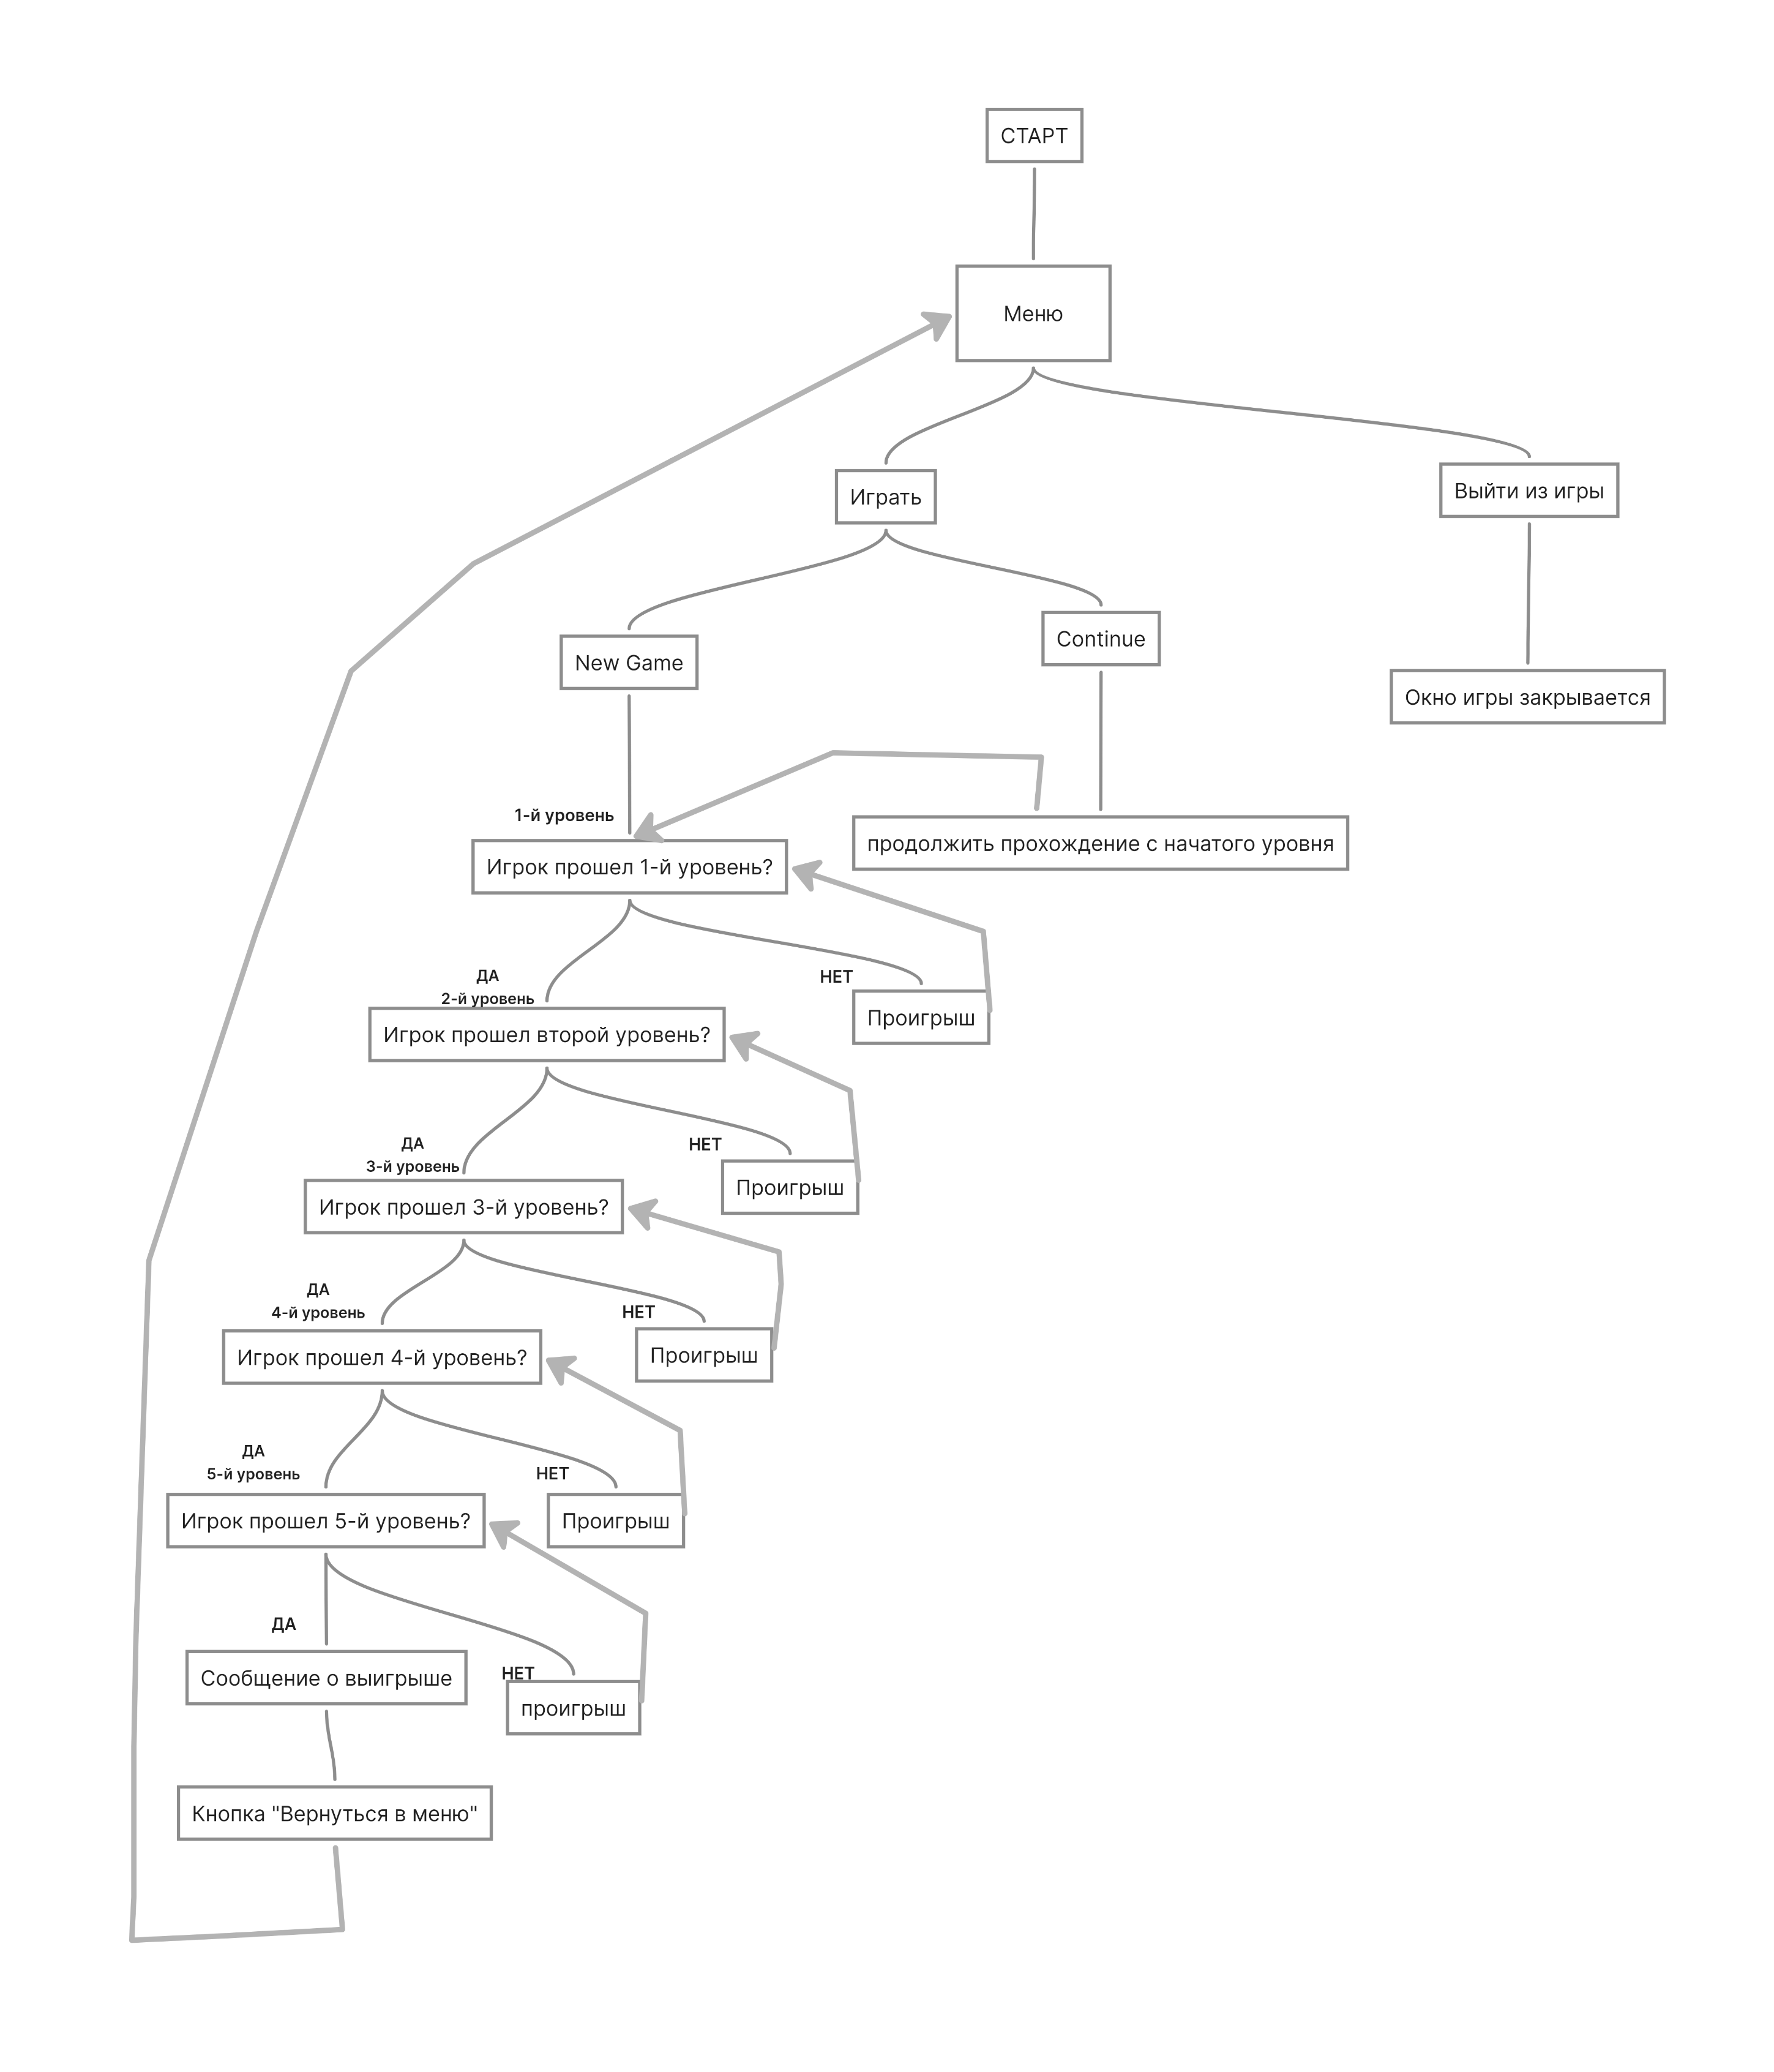
\includegraphics[width=1.0\linewidth]{схема.png}
    \caption{Блок-схема игры-платформера "HSE" на Unity}
    \label{fig:mpr}
    \end{figure}
    \end{itemize}
\subsubsection{Функциональное описание и управление}
    Функциональный интерфейс состоит из следующих экранов:
    \begin{enumerate}
  \item \textbf{Экран меню} \par
      Предоставляет пользователю интерфейс для управления игровым процессом. Позволяет начинать игру, запускать с последнего сохранения, завершать игру с последующим выходом.
  \item \textbf{Экран игрового процесса} \par
      Предоставляет пользователю интерфейс для взаимодействия с игровым процеесом. Позволяет управлять персонажем, взаимодействовать с игровым окружением, возвращаться в главное меню.
  \item \textbf{Финальный экран}\par
      Информирует пользователя об успешном прохождении игры и предоставляет интерфейс для выхода в меню.
    \end{enumerate}
\subsubsection{Объекты интерфейса пользователя}
    \begin{enumerate}
    \item \textbf{Кнопки в главном меню:}  
    Главный экран содержит следующие кнопки:  
    \begin{itemize}
        \item \textbf{Начать игру:} запускает новую игру с самого начала.  
        \item \textbf{Продолжить:} загружает последнее сохранение.  
        \item \textbf{Выход:} завершает игру и закрывает приложение.  
    \end{itemize}

    \item \textbf{Кнопки на каждом уровне:}  
    На каждом уровне в правом верхнем углу экрана отображается кнопка:  
    \begin{itemize}
        \item \textbf{Возврат в главное меню:} позволяет игроку выйти из текущего уровня и вернуться в главное меню. При нажатии на эту кнопку прогресс текущего уровня не сохраняется.  
    \end{itemize}

    \item \textbf{Финальный экран:}  
    После завершения игры появляется простой экран с текстом, уведомляющим игрока об окончании игры.  
    \begin{itemize}
        \item \textbf{Кнопка возврата в меню:} позволяет игроку вернуться в главное меню для повторного прохождения или выхода из игры.  
    \end{itemize}
    \end{enumerate}
\subsection{Графика и видео}

\subsubsection{Общее описание}
    \begin{enumerate}
    \item \textbf{Техническое исполнение} \par
    Графика игры выполнена в 2D формате. В игре детально проработаны модели и анимации персонажей, так как каждый элемент игры отрисован вручную. Использование векторной графики позволило сделать линии более чёткими и масштабировать модели без потери качества.
    \item\textbf{Стилистика, атмосфера и палитра} \par
    Графический стиль игры базируется на карикатурной идее, поэтому игра ощущается легко и позитивно. Яркий и насыщенный белый фон влекёт за собою внимание и погружает игрока в живую среду студента Вышки. А на контрасте с тёмным кирпичом даёт понять игроку, что путь его ждёт не простой. Анимации персонажей усиливают чувство динамичности игры.
    \item \textbf{Другие общие сведения} \par
    Графика в игре сочетает в себе элементы платформера и стратегии. Сочетание платформера и стратегии в графическом исполнении однозначно придаёт проекту уникальности и разнообразия. Визуальные элементы платформера, такие как блочные структуры и препятствия, чётко выделены и легко воспринимаются. Это позволяет игрокам быстро ориентироваться в пространстве и строить стратегии для преодоления препятствий. Анимации врагов и персонажей проработаны таким образом, чтобы игрок мог предугадывать их действия. Динамичность анимации делает игру более захватывающей — сражения с врагами превращаются в живое представление.
    \end{enumerate}

\subsubsection{Двумерная графика и анимация}
    В данном разделе описана основная 2D графика и анимация, которые необходимо разработать для игры.
    \begin{enumerate}
    \item \textbf{Интерфейс}
    В игре реализовано меню с возможностью начать новую игру или продолжить с того места, где игрок остановился. Также предусмотрена опция выхода из игры с автосохранением. Интерфейс выполнен в минималистичном, но интуитивно понятном стиле. Управление персонажем осуществляется с помощью клавиш \texttt{WASD} или стрелок на клавиатуре, взаимодействие с меню — через курсор мыши.

    \item \textbf{Эффекты}
    При уничтожении врагов происходит эффект их мгновенного исчезновения. Также при попадании снарядов противника в игрока, тот моментально выводится из игры, что сопровождается визуальным эффектом.

    \item \textbf{Персонажи, строения и юниты}
    Для моделей персонажей, противников и уровней использована векторная графика. Нарисовано: 1 главный герой, 12 различных противников, 1 босс, блоки для генерации уровня и фоновая заставка. Персонаж имеет анимацию передвижения и прыжков.

    \item \textbf{Игровой мир}
    Игровой мир выполнен в светлых тонах: стены корпуса Вышки имеют белый цвет, а пол и потолок — тёмные оттенки кирпича.
    \end{enumerate}
\subsubsection{Трехмерная графика и анимация}

\subsubsection{Анимационные вставки}

\subsection{Звуки и музыка}

\subsubsection{Общее описание}
    \begin{enumerate}
    \item \textbf{Характер музыкальных тем} \par
    Каждый уровень игры приурочен к определенному курсу обучения, поэтому музыкальное сопровождение варьируется в зависимости от темы и настроения, соответствующего выбранному курсу. Например, для первого уровня, который может представлять собой вводный курс, музыка будет легкой и мелодичной, с элементами оптимизма и надежды. По мере продвижения к более сложным курсам, музыкальные темы становятся более напряжёнными и сложными. На втором и третьем уровнях звуки производят ощущение давления испытываемое студентами.
    \item\textbf{Создаваемое настроение} \par
    С каждой новой темой углубляется и эмоциональная нагрузка игры. Четвертый уровень, где студенты сталкиваются с более серьезными испытаниями, сопровождён мрачной и загадочной музыкой. Здесь игрок может ощутить важность своих решений, когда каждая ошибка может стать фатальной. Финальный уровень, посвященный защите диплома, будет являться кульминацией, а потому здесь присутствуют эпические звучания и динамичные ритмов. Перед лицом диплома, музыка поднимется до максимальной напряжённости.
    \item \textbf{Насыщенность мира звуками} \par
    Звуковая палитра игры обогащена многочисленными звуковыми эффектами: шаги по коридорам университета, оплеухи врагов и победы над ними. В каждом уровне используются свои уникальные звуки. Отдельное внимание уделяется эффектам, возникающим в моменты столкновения с врагами, например, различные звуки для «попадания» и «неудачи».
    \end{enumerate}

\subsubsection{Звук и звуковые эффекты}
    Звуки интерфейса обеспечивают обратную связь с игроком и делают взаимодействие с меню и элементами HUD более интуитивным. \\
Примеры звуков и их использование:
    \begin{enumerate}
    \item \textbf{Звуки интерфейса}
    \begin{itemize}
        \item Клик по кнопке в меню — короткий щелчок или звенящий звук, сопровождающий выбор элемента.
        \item Подтверждение действия — мягкий звук, подчеркивающий успешное выполнение (например, старт игры или сохранение).
        \item Ошибка или недоступное действие — короткий низкий звук, информирующий игрока о невозможности выполнить действие.
        \item Сбор ресурсов (монеты, очки) — звуковой сигнал, сопровождающий изменение числовых значений на экране.
        \item Звуки паузы/возобновления игры — приглушенные или нарастающие звуки, подчеркивающие переход между игровыми и неигровыми состояниями.
    \end{itemize}
    \item \textbf{Звуки спецэффектов}
    \begin{itemize}
        \item Удар или столкновение — резкие звуки, зависящие от материала объектов, участвующих в столкновении.
        \item Смерть врага — уникальные звуки, подчеркивающие характер каждого типа врага.
    \end{itemize}
    \item \textbf{Звуки игровых объектов}
    \begin{itemize}
        \item Движение персонажа — звуки шагов с учетом поверхности.
        \item Прыжки — короткие, упругие звуки, сопровождающие момент отталкивания от земли
        \item Ловушки — звуки активации (например, щелчок механизма, свист летящего объекта или металлический лязг).
    \end{itemize}
    \end{enumerate}
\subsubsection{Музыка}
    \begin{enumerate}
    \item \textbf{Главный интерфейс новой игры:}  
    Для главного меню используется спокойная и расслабляющая мелодия с элементами фортепиано и синтезатора, создающая атмосферу ожидания. Она напоминает шум библиотеки или уютной аудитории, чтобы подчеркнуть тематику студенческой жизни.  

    \item \textbf{Музыкальное сопровождение роликов:}  
    \begin{itemize}
        \item \textbf{Начальный ролик:} динамичная композиция с нарастающим темпом, символизирующая вступление в студенческую жизнь и её вызовы.  
        \item \textbf{Финальный ролик (победа):} торжественная мелодия, включающая элементы фанфар, символизирующая успешное завершение всех испытаний.  
        \item \textbf{Финальный ролик (поражение):} меланхоличная мелодия с использованием медленных струнных инструментов, передающая чувство упущенной возможности.  
    \end{itemize}

    \item \textbf{Состав тем по уровням игры:}  
    Каждый уровень имеет свою уникальную музыкальную тему, отражающую его содержание:  
    \begin{itemize}
        \item \textbf{Уровень 1:} бодрая, слегка хаотичная мелодия с элементами джаза и электронного звучания, символизирующая хаос первого курса.  
        \item \textbf{Уровень 2:} мелодия средней интенсивности с элементами гитарного сопровождения, подчёркивающая постепенное усложнение учебного процесса.  
        \item \textbf{Уровень 3:} напряжённая и ритмичная электронная композиция, отражающая интеллектуальные испытания, связанные с курсами Machine Learning и контестами.  
        \item \textbf{Уровень 4:} атмосферная и мрачная мелодия с элементами хора и низких струнных инструментов, подчеркивающая стресс последнего курса.  
        \item \textbf{Уровень 5 (Босс):} эпичная мелодия с элементами ударных, создающая напряжение и подталкивающая игрока к финальной битве.  
    \end{itemize}

    \item \textbf{Особенные фрагменты:}  
    \begin{itemize}
        \item \textbf{Action-сцены:} динамичные треки с ускоряющимся темпом и мощными ударными для создания напряжённой атмосферы в сражениях.  
        \item \textbf{Отрицательный финал:} мелодия с преобладанием пианино и низких струнных инструментов, передающая чувство разочарования.  
        \item \textbf{Победа над боссом:} короткая, но торжественная мелодия с использованием фанфар и высоких струнных инструментов, чтобы подчеркнуть триумф игрока.  
    \end{itemize}
    \end{enumerate}

    \textbf{Общее содержание:}  
    Музыкальные треки написаны в стилях, сочетающих элементы электроники, классической музыки и джаза, чтобы поддерживать тематическую связь с игровой атмосферой. Каждый трек адаптирован под соответствующий игровой контекст и усиливает впечатления от происходящего.
\subsection{Описание уровней}

\subsubsection{Общее описание дизайна уровней}
    \begin{itemize}
    \item \textbf{Общее описание} \par
    Дизайн игры тесно связан с HSE, поэтому многие игровые элементы стилизованы под университетскую среду. 
    Игровой процесс построен таким образом, чтобы каждый уровень был уникальным и символизировал различные этапы образовательного пути студента. 
    Каждый новый этап будет увеличивать сложность и разнообразие задач, противников и препятствий. В свою очередь, каждый уровень будет продвигать сюжет вперед и раскрывать новые аспекты.

    \item \textbf{Ключевые критерии дизайна уровней} \par
    Дизайн уровней имеет прямую связь с HSE. В зависимости от тематики каждого этапа, дизайн уровней будет изменяться, используя различные визуальные стили для отображения изменений в образовательной среде.
    На начальных уровнях акцент будет на учебных аудиториях, а на более поздних — на библиотеках, лабораториях, административных помещениях.
    \end{itemize}
\subsubsection{Диаграмма взаимного расположения уровней}
    \begin{itemize}
    \item \textbf{Диаграмма взаимного расположения уровней} \\
    В данной игре уровни представляют собой последовательные курсы обучения в ВШЭ, расположенные по линейно-последовательной схеме, где каждый уровень содержит свои уникальные враги, усложняющие жизнь студентов. Успешное преодоление всех уровней ведет к ключевой локации - пятому уровню - финальному сражению с дипломом.
    Игра содержит в себе следующие уровни:
    \begin{itemize}
        \item Первый курс
        \\Враги: Оценка "-10", интеграл, Smart LMS
        \item Второй курс
        \\Враги: Английский язык, Python, теория вероятностей и математическая статистика
        \item Третий курс
        \\Враги: Machine Learning, Яндекс Контест, курсовая работа
        \item Четвёртый курс
        \\Враги: Философия, значок Яндекс Почты с непрочитанными письмами, вышкинская ворона
        \item Финальный уровень
       \\ Босс: Диплом
    \end{itemize}
    Каждый уровень увеличивает сложность и добавляет новые вызовы на пути студента, что создает интересный игровой процесс.
    \end{itemize}

\subsubsection{График введения новых объектов}
    \begin{enumerate}
    \item \textbf{Общее построение усложнения игры} \par
    С каждым уровнем (курсом) игрок сталкивается с уникальными врагами и механиками, которые соответствуют тематике этого этапа обучения. Враги становятся более сложными, требуют разных стратегий для победы, что мотивирует игрока учиться на своих ошибках. Сначала враги имеют простой набор атак, но с каждым уровнем их поведение усложняется (например, враги второго курса могут использовать полет и стрельбу, а враги третьего курса требуют стратегического подхода).С каждым уровнем игрок открывает новую упаковку успокоительного, чтобы компенсировать растущую сложность.
    \item\textbf{Подробный график введения объектов} \par
    Первый курс: \par
    • Введение базовых механик и врагов. \par Smart LMS \par
    Второй курс: \par
    • Усложнение боя с использованием новых типов врагов. \par
    Третий курс: \par
    • Введение мини-боссов и этапов подготовки к финальному бою. \par
    Четвёртый курс: \par
    • Кульминация развития врагов и создание условий высокого давления. \par
    Финальный уровень – диплом: \par
    • Босс, объединяющий в себе механики всех предыдущих врагов. \par
    \item\textbf{Поддержание интереса}
    Игрок получает награды за прохождение уровней, например, улучшения навыков или полезные предметы. Это мотивирует продолжать игру. Каждая “аудитория” (уровень) имеет уникальный дизайн, усиливающий погружение в мир. График введения новых объектов обеспечивает плавное усложнение и поддержание интереса игрока на каждом этапе игры, постепенно подводя его к финальному сражению.
    \end{enumerate}

\section{Контакты}
    \item \textbf{Контактные лица:} \par
    Высоцкий Леонид Дмитриевич \par
    Сапрыкин Николай Андреевич \par
    Гусев Егор Александрович \par
    Шепшелюк Анастасия Алексеевна \par
    Цирулёв Дмитрий Александрович \par
    Троицкий Никита Александрович \par
    \item \textbf{Телефоны:} \par
    89506182676 (Дмитрий) \par
    89736016835 (Леонид) \par
    89501638642 (Николай) \par
    89356926841 (Егор) \par
    89835833977 (Анастасия) \par
    89206947693 (Никита) \par
    \item \textbf{Email:} \par
    datsirulev@edu.hse.ru (Дмитрий)
    \item \textbf{Адрес:} \par
    ул. Космическая улица, 44, Нижний Новгород, 603142
    \item \textbf{Сайт:} \par
    https://github.com/DmitriyHSE/projectUnity
\end{document}

